The Pre-Thesis~II report made three kinds of claim that this chapter re-examines:
that learned fusion outperforms naive late fusion within-subject, with a
state-of-the-art result on EAV; that the three modalities' trials are aligned; and
that the suppression matrix reveals population-level patterns of emotion suppression.
Each was re-tested with a procedure designed to be able to refute it. The first is
weakened, the second is found to be unverifiable from the available data, and the
third does not survive. The chapter reports all three in full, because the audit is
itself a contribution: every test it uses is cheap, reusable, and applicable to other
work on this benchmark.

The corrected figures are the ones used throughout this report. Chapter~\ref{chap:within}
reports the leak-free within-subject results, and this chapter explains how they
differ from the Pre-Thesis~II figures and why.

\section{Model Selection on the Test Set}
\label{sec:audit_selection}

\subsection{The Defect}

All three Pre-Thesis~II fusion scripts---\texttt{day5\_pipeline.py} (cross-attention),
\texttt{concat\_mlp\_baseline.py} and \texttt{day7\_modality\_dropout.py}---evaluated
the fusion head on each participant's 120 test trials after every one of 80 training
epochs and kept the best. The reported accuracy for each participant was therefore the
maximum of 80 measurements on the test set. The report described this openly as
``best-test-epoch checkpointing'', but did not treat it as a source of bias.

It is one. The maximum of many noisy measurements is biased upward, and on 120 test
trials a single trial moves accuracy by 0.83 points. Selecting a model on the data used
to evaluate it is a well-documented source of optimistic bias in cross-validated
estimates \cite{Varma2006CVBias,Cawley2010Overfitting} and in neuroscience analysis
more broadly \cite{Kriegeskorte2009DoubleDipping}. The bias here is also asymmetric:
naive late fusion has no epochs to select from, so it received no such boost. The
Pre-Thesis~II comparison of learned fusion against averaging was therefore tilted in
favour of learned fusion.

The per-modality encoders are not affected. The EAV trainers train for a fixed number of
epochs and keep the final state; test accuracy is printed but never used to choose
weights. The per-modality accuracies (57.1\%, 74.6\%, 43.9\%) and naive late fusion
(77.5\%) are therefore free of test-set selection. One weaker form of test exposure
remains: the per-modality epoch budgets were reduced after inspecting three pilot
participants' training curves (Section~\ref{sec:epoch_budget}). This affects three
hyperparameters chosen once, not a per-participant choice, and is disclosed rather
than corrected.

\subsection{Leak-Free Re-Evaluation}

\texttt{p2\_leakfree.py} reproduces the Pre-Thesis~II recipe exactly---the same cached
within-subject features, AdamW at learning rate $10^{-3}$ with weight decay
$10^{-4}$, cosine annealing, batch size 32, 80 epochs, softhard dropout at $p = 0.5$---and
changes only how the reported epoch is chosen. Each head is trained twice per
participant:
\begin{itemize}
  \item \textbf{Run A} fits on a stratified 80\% of the 280 training trials (224),
  holding out the other 56 as a validation set. The single training trajectory is read
  out three ways: \emph{test-selected} (best test accuracy over the 80 epochs, the
  Pre-Thesis~II protocol), \emph{validation-selected} (test accuracy at the epoch of
  best validation accuracy), and \emph{final-fit} (test accuracy at the last epoch).
  Because all three readouts come from the same weights, the difference between
  test-selected and validation-selected is the selection inflation itself, not a
  difference between two runs.
  \item \textbf{Run B} fits on all 280 training trials for the fixed 80 epochs and
  reports the final epoch, with no selection of any kind: \emph{final-full}.
\end{itemize}

Final-full was designated the primary figure before the results were inspected. It is
the natural end point of the recipe (the cosine schedule anneals the learning rate to
zero at epoch 80), it trains on the same 280 trials as the Pre-Thesis~II heads and as
the encoders feeding naive late fusion, and it involves no choice that could be
influenced by any held-out data.

\begin{table}[htbp]
\centering
\small
\caption{Within-subject fusion accuracy under each readout, mean over 42
participants. ``P2'' is the figure published in the Pre-Thesis~II report. Inflation is
test-selected minus validation-selected on the same Run~A trajectory. Naive late
fusion is 77.48\% throughout.}
\label{tab:audit_leakfree}
\begin{tabular}{lcccccc}
\hline
\textbf{Head} & \textbf{P2} & \textbf{Test-sel.} & \textbf{Val-sel.} & \textbf{Final-fit} & \textbf{Final-full} & \textbf{Inflation} \\
\hline
Cross-attention         & 80.2\% & 81.43\% & 75.65\% & 77.72\% & 76.75\% & $+5.77$ pp \\
Concat-MLP              & 81.7\% & 81.65\% & 76.39\% & 79.09\% & 79.96\% & $+5.26$ pp \\
Modality dropout (full) & 84.7\% & 83.61\% & 76.13\% & 78.04\% & 79.80\% & $+7.48$ pp \\
Modality dropout (AV)   & 81.5\% & 81.37\% & 75.04\% & 77.52\% & 79.17\% & $+6.33$ pp \\
\hline
\end{tabular}
\end{table}

Table~\ref{tab:audit_leakfree} gives the result. The rerun reproduces the published
protocol closely: its test-selected concat-MLP figure is 81.65\% against the published
81.7\%. The other test-selected figures differ from the published ones by up to 1.2
points, because Run~A fits on 224 rather than 280 trials and the epoch maximum is a
noisy statistic. The selection inflation is 5.3 to 7.5 points, and it is largest for the
modality-dropout head, plausibly because its training curve is the noisiest: every
batch randomly removes modalities, so test accuracy fluctuates more from epoch to epoch
and its maximum is further from its typical value.

Validation-selected is the lowest readout for every head, below even final-fit. With
56 validation trials, the choice of epoch is itself noisy enough to pick worse epochs
than simply stopping at the end; this is the same phenomenon documented at fold scale
in Section~\ref{sec:cs_challenges} (C17). It supports the a-priori choice of final-full
as the primary readout.

\subsection{Corrected Comparisons}

Table~\ref{tab:within_tests} in Chapter~\ref{chap:within} gives the corrected comparisons. Two findings are robust.
Plain cross-attention does \emph{not} beat naive late fusion ($-0.73$ points); the
Pre-Thesis~II claim that it did ($+2.7$ points, $p = 0.023$) was produced by test-set
selection. And both modality dropout and concat-MLP beat plain cross-attention by
about three points on the leak-free readout, significantly after correction.

Whether concat-MLP and the dropout model beat naive late fusion depends on the test
family, and is therefore reported as marginal. Their raw $p$-values are 0.0063 and
0.0085. Corrected over the four primary head-versus-naive tests, both give
$p_{\mathrm{Holm}} = 0.025$; over the 7-test family of Table~\ref{tab:within_tests},
0.031 and 0.034; over the 8-test family that also includes the validation-selected
readouts, 0.050 and 0.059. A gain of about 2.4 points that crosses the conventional
threshold under some reasonable corrections and not others is not a finding to build a
thesis on, and it is not used as one.

Two further comparisons concern the zero-EEG path, tested as a separate two-test
family. With EEG zeroed at inference, the dropout model (79.17\%) still beats
full-modality cross-attention (76.75\%) by 2.42 points (26 of 42 participants;
$p_{\mathrm{Holm}} = 0.0043$). Removing EEG from the dropout model costs 0.63 points,
which is not significant ($p_{\mathrm{Holm}} = 0.16$).

\subsection{Consequences for the Pre-Thesis~II Claims}

\textbf{The state-of-the-art claim is withdrawn.} Pre-Thesis~II reported 84.7\% for
the dropout model, 8.05 points above the best published EAV fusion result (Hyper-MML,
76.65\% \cite{Kang2025HyperMML}). The leak-free figure is 79.8\%. It remains
numerically above the published comparators, but no state-of-the-art claim is made,
for two reasons. The comparators do not report how their epochs or checkpoints were
selected, so it cannot be established that the protocols are comparable; and
Chapters~\ref{chap:crosssubject} and~\ref{chap:calibration} show that within-subject
accuracy on EAV is substantially driven by participant identity, which makes
within-subject rankings a weak basis for any such claim.

\textbf{The ranking of heads survives; the size of the dropout effect shrinks.}
Pre-Thesis~II reported modality dropout as a 4.5-point gain over cross-attention; the
leak-free gain is 3.1 points, still highly significant.

\textbf{The zero-EEG path survives.} The claim that the dropout model
without EEG beats cross-attention with EEG is, if anything, stronger after correction.

\section{Trial Alignment}
\label{sec:audit_alignment}

Every trimodal model and every coherence analysis in this thesis compares audio trial
$i$, vision trial $i$ and EEG trial $i$ as if they were the same interaction. The
Pre-Thesis~II report supported this with a per-class count check
(Section~\ref{sec:split_alignment}): every participant has 80 trials per class in
every modality. That is a necessary condition, but a weak one; any ordering with 80
trials per class passes it.

\texttt{label\_sequence\_check.py} tests the stronger condition: that the label
\emph{sequences} match element by element across the three modalities, for the
training and test split of every participant (84 splits). It also reports whether that
check can be informative, by counting the number of label changes along each sequence.
If the labels are sorted into class blocks, the sequences match trivially and say
nothing about whether trial $i$ is the same interaction in each modality.

The result is that all 84 splits match element-wise, and all 84 are class-blocked: every
label sequence consists of five contiguous runs, one per class. The match is therefore
guaranteed by the blocking and is uninformative. \textbf{Trial correspondence within a
class is unverified}, and it cannot be verified from the released pickles, which carry
no trial identifiers.

Two points limit the damage. First, the fusion accuracies do not depend on it: a head
trained and tested on same-class tuples of clips is still a valid classifier of such
tuples, even if the clips in a tuple came from different interactions. What is lost is
the claim that the tuple is one moment of one person's behaviour. Second, the EEG and
the audio-visual signals were never simultaneous in the first place: EAV's EEG is
taken from the listening window and the audio and video from the speaking window
(Section~\ref{sec:listenspeak_asymmetry}). Trial-level analyses---the suppression
matrix above all---are the ones that depend on alignment, and Section~\ref{sec:audit_suppression}
finds one piece of indirect evidence that the pairing carries shared trial-level
structure.

\section{The Suppression Matrix}
\label{sec:audit_suppression}

\subsection{The Pre-Thesis~II Analysis}

The suppression matrix counts trials on which audio and vision agree on an emotion
(external consensus), EEG predicts a different emotion, and EEG's top-1 probability is
at least 0.5 (Section~\ref{sec:coherence_analysis}). Over the 5{,}040 within-subject test
trials it contains 401 such events, an 8.0\% base rate (Table~\ref{tab:suppression_matrix}).

\begin{table}[htbp]
\centering
\small
\caption{Within-subject suppression matrix, 42 participants, 5{,}040 test trials. Rows:
audio-vision consensus. Columns: EEG prediction. Total 401 events.}
\label{tab:suppression_matrix}
\begin{tabular}{l c c c c c}
\hline
\textbf{Consensus / EEG} & \textbf{Neutral} & \textbf{Sadness} & \textbf{Anger} & \textbf{Happiness} & \textbf{Calmness} \\
\hline
Neutral   & 0  & 5  & 3  & 8  & 24 \\
Sadness   & 43 & 0  & 21 & 12 & 20 \\
Anger     & 5  & 13 & 0  & 65 & 10 \\
Happiness & 11 & 17 & 52 & 0  & 14 \\
Calmness  & 40 & 17 & 4  & 17 & 0 \\
\hline
\end{tabular}
\end{table}

Pre-Thesis~II read three patterns from this matrix as population-level signatures of
affective incoherence: a bidirectional Anger--Happiness pattern (65 and 52 events),
interpreted as shared high-arousal physiology; Sadness$\rightarrow$Neutral (43),
interpreted as suppression of sadness; and Calmness$\rightarrow$Neutral (40). It
checked that the patterns were spread across participants and that EEG's tendency to
predict Neutral was not inflated among the events.

Neither check addresses the obvious alternative. EAV is cue-based: the participant is
told which emotion to express, and audio and vision usually get it right. When they
agree, their consensus is usually the cued label. A ``suppression event'' is then
mostly a trial on which EEG made a confident error on a trial the audio-visual
classifiers got right, and the matrix is EEG's confusion matrix seen through a filter.
If so, the patterns describe EEGNet, not the participants.

\subsection{Three Tests}

\texttt{suppression\_audit.py} tests this alternative in three steps.

\textbf{(a) Consensus correctness.} On 352 of the 401 events (87.8\%), the audio-vision
consensus equals the cued label. The rows of the matrix are, overwhelmingly, the true
classes, and the events are EEG errors on those classes.

\textbf{(b) Resemblance to EEG's own errors.} The 20 off-diagonal cells of the matrix
correlate with EEG's confident-error confusion matrix (errors at confidence $\ge 0.5$)
at $r = 0.956$ over all trials and $r = 0.989$ over trials that audio-vision classified
correctly. The matrix reproduces what EEG gets wrong regardless of what the other
modalities do.

\textbf{(c) Class-conditional permutation null.} This is the decisive test. Within
each participant and each cued class, EEG's (prediction, confidence) pairs are shuffled
across trials while audio and vision are held fixed, and the matrix is recomputed; this
is repeated 2{,}000 times. The shuffle preserves every classifier's per-class accuracy
and confusion pattern exactly and destroys only the trial-level pairing between the
audio-visual and EEG predictions. If the observed matrix lies inside the resulting null
distribution, the events carry no trial-level coupling beyond what independent,
class-conditional errors produce. Two-sided permutation $p$-values are computed as
$(b + 1)/(m + 1)$ for $b$ exceedances in $m$ permutations \cite{Phipson2010Permutation},
with Holm correction over the 20 cells. Before use, the test was checked on synthetic
data: it is silent when errors are generated independently and detects coupling when
it is planted.

\begin{figure}[htbp]
\centering
\IfFileExists{images/fig_audit_suppression.png}{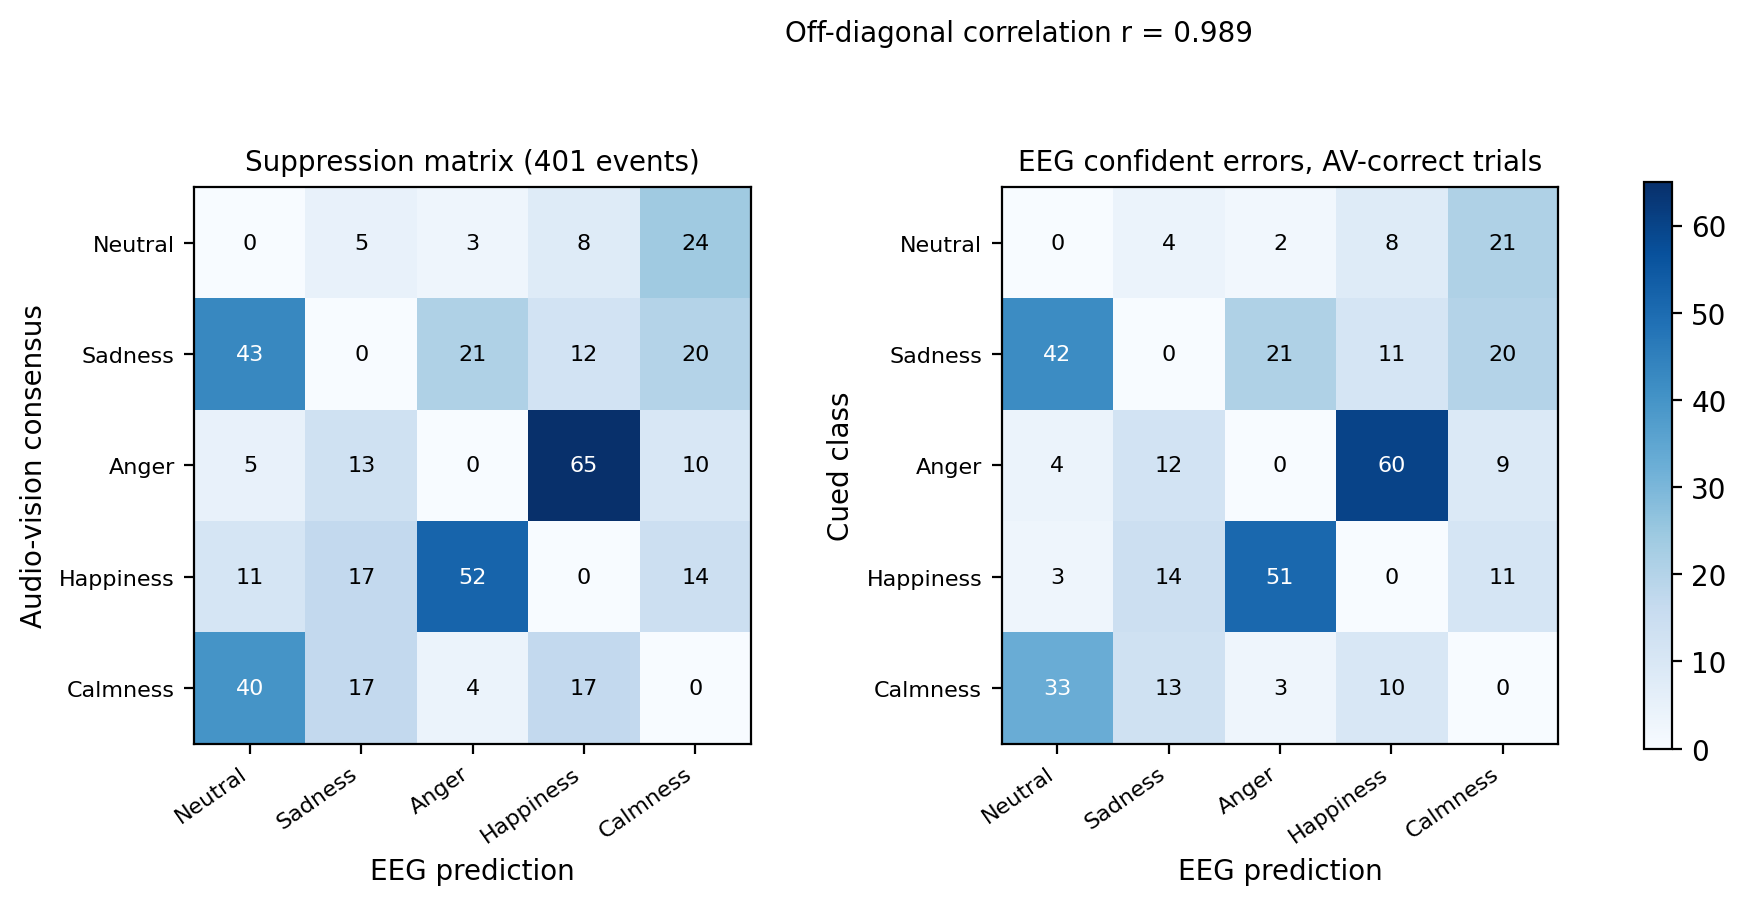
\includegraphics[width=0.95\textwidth]{images/fig_audit_suppression.png}}{\fbox{\parbox{0.9\textwidth}{\centering Missing image placeholder: \texttt{images/fig\_audit\_suppression.png} (left: within-subject suppression matrix; right: EEG confident-error matrix on audio-vision-correct trials; same colour scale).}}}
\caption{The within-subject suppression matrix (left) beside EEG's confident-error
confusion matrix on trials audio and vision classified correctly (right). Off-diagonal
correlation $r = 0.989$.}
\label{fig:audit_suppression}
\end{figure}

\textbf{Result.} No cell of the within-subject matrix differs from the null after
correction. The patterns Pre-Thesis~II interpreted are fully accounted for by each
classifier's class-conditional error rates. The total number of events differs from
the null, but in the opposite direction to suppression: 401 observed against
$436.8 \pm 12.4$ expected ($p = 0.005$). Confident EEG disagreement co-occurs with
audio-visual consensus \emph{less} often than independent errors would produce; the
modalities tend to be right, and wrong, on the same trials.

That last result is the indirect alignment evidence promised in
Section~\ref{sec:audit_alignment}. The within-class shuffle removes any dependence
between modalities that is carried by the trial pairing, so a significant departure
from the null shows that the pairing carries shared structure---trial difficulty,
recording drift, or genuinely shared affect. It does not prove that trial $i$ is the
same interaction in every modality, but it is not what an arbitrary pairing would
produce.

\subsection{Cross-Subject Replication}

The same audit was run on the cross-subject logits of Chapter~\ref{chap:crosssubject},
16{,}800 trials from encoders that never saw the participant
(Table~\ref{tab:audit_cross}).

\begin{table}[htbp]
\centering
\small
\caption{Cross-subject suppression matrix, 42 participants, 16{,}800 held-out trials.
Total 621 events (3.7\% base rate).}
\label{tab:audit_cross}
\begin{tabular}{l c c c c c}
\hline
\textbf{Consensus / EEG} & \textbf{Neutral} & \textbf{Sadness} & \textbf{Anger} & \textbf{Happiness} & \textbf{Calmness} \\
\hline
Neutral   & 0  & 5  & 39  & 29  & 1 \\
Sadness   & 69 & 0  & 39  & 66  & 0 \\
Anger     & 10 & 21 & 0   & 186 & 0 \\
Happiness & 2  & 3  & 88  & 0   & 2 \\
Calmness  & 23 & 0  & 10  & 28  & 0 \\
\hline
\end{tabular}
\end{table}

The picture is the same. The consensus equals the cued label on 78.3\% of the 621
events; the matrix correlates with EEG's confident-error matrix at $r = 0.871$ (all
trials) and $r = 0.985$ (audio-vision-correct trials); and the total is again below the
null (621 against $680.7 \pm 14.9$, $p = 0.0005$). Two cells differ from the null after
Holm correction. Happiness$\rightarrow$Anger is \emph{below} it (88 against 112.5,
$z = -3.75$, $p_{\mathrm{Holm}} = 0.010$). Sadness$\rightarrow$Neutral is above it (69
against 51.2, $z = +4.49$, $p_{\mathrm{Holm}} = 0.010$).

Sadness$\rightarrow$Neutral is the only cell anywhere in this thesis in which
audio-visual/EEG disagreement exceeds what independent errors predict. It is
nonetheless a candidate rather than a finding: it is one cell out of 40 tested across
the two protocols, it does not replicate within-subject, and the EAV design offers no
independent measure of what the participant felt. It is recorded as a hypothesis for a
study with concurrent self-report.

\subsection{Verdict}

The suppression matrix does not support claims of emotion suppression on EAV. Within
subject, it is statistically indistinguishable from the matrix that EEG's own
class-conditional errors would produce, and the Anger--Happiness pattern in particular
is EEGNet's confusion between two high-arousal classes, not a property of the
participants. RQ4 is answered accordingly in Section~\ref{sec:audit_rq}.

What survives is methodological. A coherence or suppression claim built from
classifier disagreement in a cue-based corpus must at minimum beat a
class-conditional permutation null of the kind used here; the test takes minutes on
cached logits, and without it such a matrix cannot be distinguished from the error
structure of its weakest classifier.

\section{Summary of the Audit}
\label{sec:audit_summary}

\begin{table}[htbp]
\centering
\small
\caption{Status of the Pre-Thesis~II claims after the audit.}
\label{tab:audit_summary}
\begin{tabular}{p{6.2cm} p{7.4cm}}
\hline
\textbf{Pre-Thesis~II claim} & \textbf{Status in this report} \\
\hline
Per-modality encoders exceed the EAV baselines & Stands. Encoders were not test-selected. \\
Naive late fusion beats vision alone within-subject & Stands. No selection involved. \\
Cross-attention beats naive late fusion ($+2.7$ pp) & Withdrawn. Leak-free $-0.73$ pp, not significant. \\
Concat-MLP beats naive late fusion ($+4.2$ pp) & Weakened to $+2.5$ pp; significance depends on the correction family. \\
Modality dropout beats cross-attention ($+4.5$ pp) & Stands at $+3.1$ pp. \\
Zero-EEG dropout path beats full cross-attention & Stands at $+2.4$ pp. \\
State of the art on EAV (84.7\%) & Withdrawn. Leak-free 79.8\%; comparators' selection protocols unknown. \\
Trial alignment verified by class counts & Unverified; the label sequences are class-blocked. \\
Suppression matrix shows population-level suppression & Not supported; matrix $\approx$ EEG error structure, inside the permutation null. \\
\hline
\end{tabular}
\end{table}

Table~\ref{tab:audit_summary} collects the outcome. The audit removes the Pre-Thesis~II
report's two most prominent claims---the state-of-the-art figure and the suppression
patterns---and replaces them with measured, smaller statements that are corrected for
multiple comparisons and robust to the choice of readout.

\section{Answers to Research Questions}
\label{sec:audit_rq}

\textbf{RQ3---Architectural contribution (within-subject), revised:} Under leak-free
evaluation, plain cross-attention fusion does not outperform naive late fusion
(76.75\% against 77.48\%). Concat-MLP and modality-dropout fusion exceed it by about
2.4 points, a margin whose significance depends on the multiple-comparison family.
Modality dropout makes the attention architecture competitive with concat-MLP (tied,
$+0.16$ points) and 3.1 points better than attention without it.

\textbf{RQ4---Coherence as signal, revised:} The suppression matrix contains the
patterns reported in Pre-Thesis~II, but they are the confusion structure of the EEG
classifier: 87.8\% of events have a correct audio-visual consensus, the matrix
correlates with EEG's own error matrix at $r = 0.989$, and no cell exceeds a
class-conditional permutation null within-subject. The modalities are more coherent at
trial level than independent errors predict, not less. A single candidate
pattern---Sadness$\rightarrow$Neutral under subject-independent evaluation---exceeds
the null and is left for a study with self-reported internal state.

\textbf{RQ9---Evaluation integrity:} Of the Pre-Thesis~II conclusions, those involving
no model selection stand; the fusion comparisons shrink by 5.3--7.5 points once
test-set epoch selection is removed; trial correspondence cannot be verified from the
released data; and the coherence patterns are not distinguishable from classifier
error. All of this was detectable with analyses of cached artefacts that take minutes
to run.
